\chapter{Sequenzdiagramme}

\section{Import von einem JOANA Graphen}

\begin{figure}[hb]
  \centering
  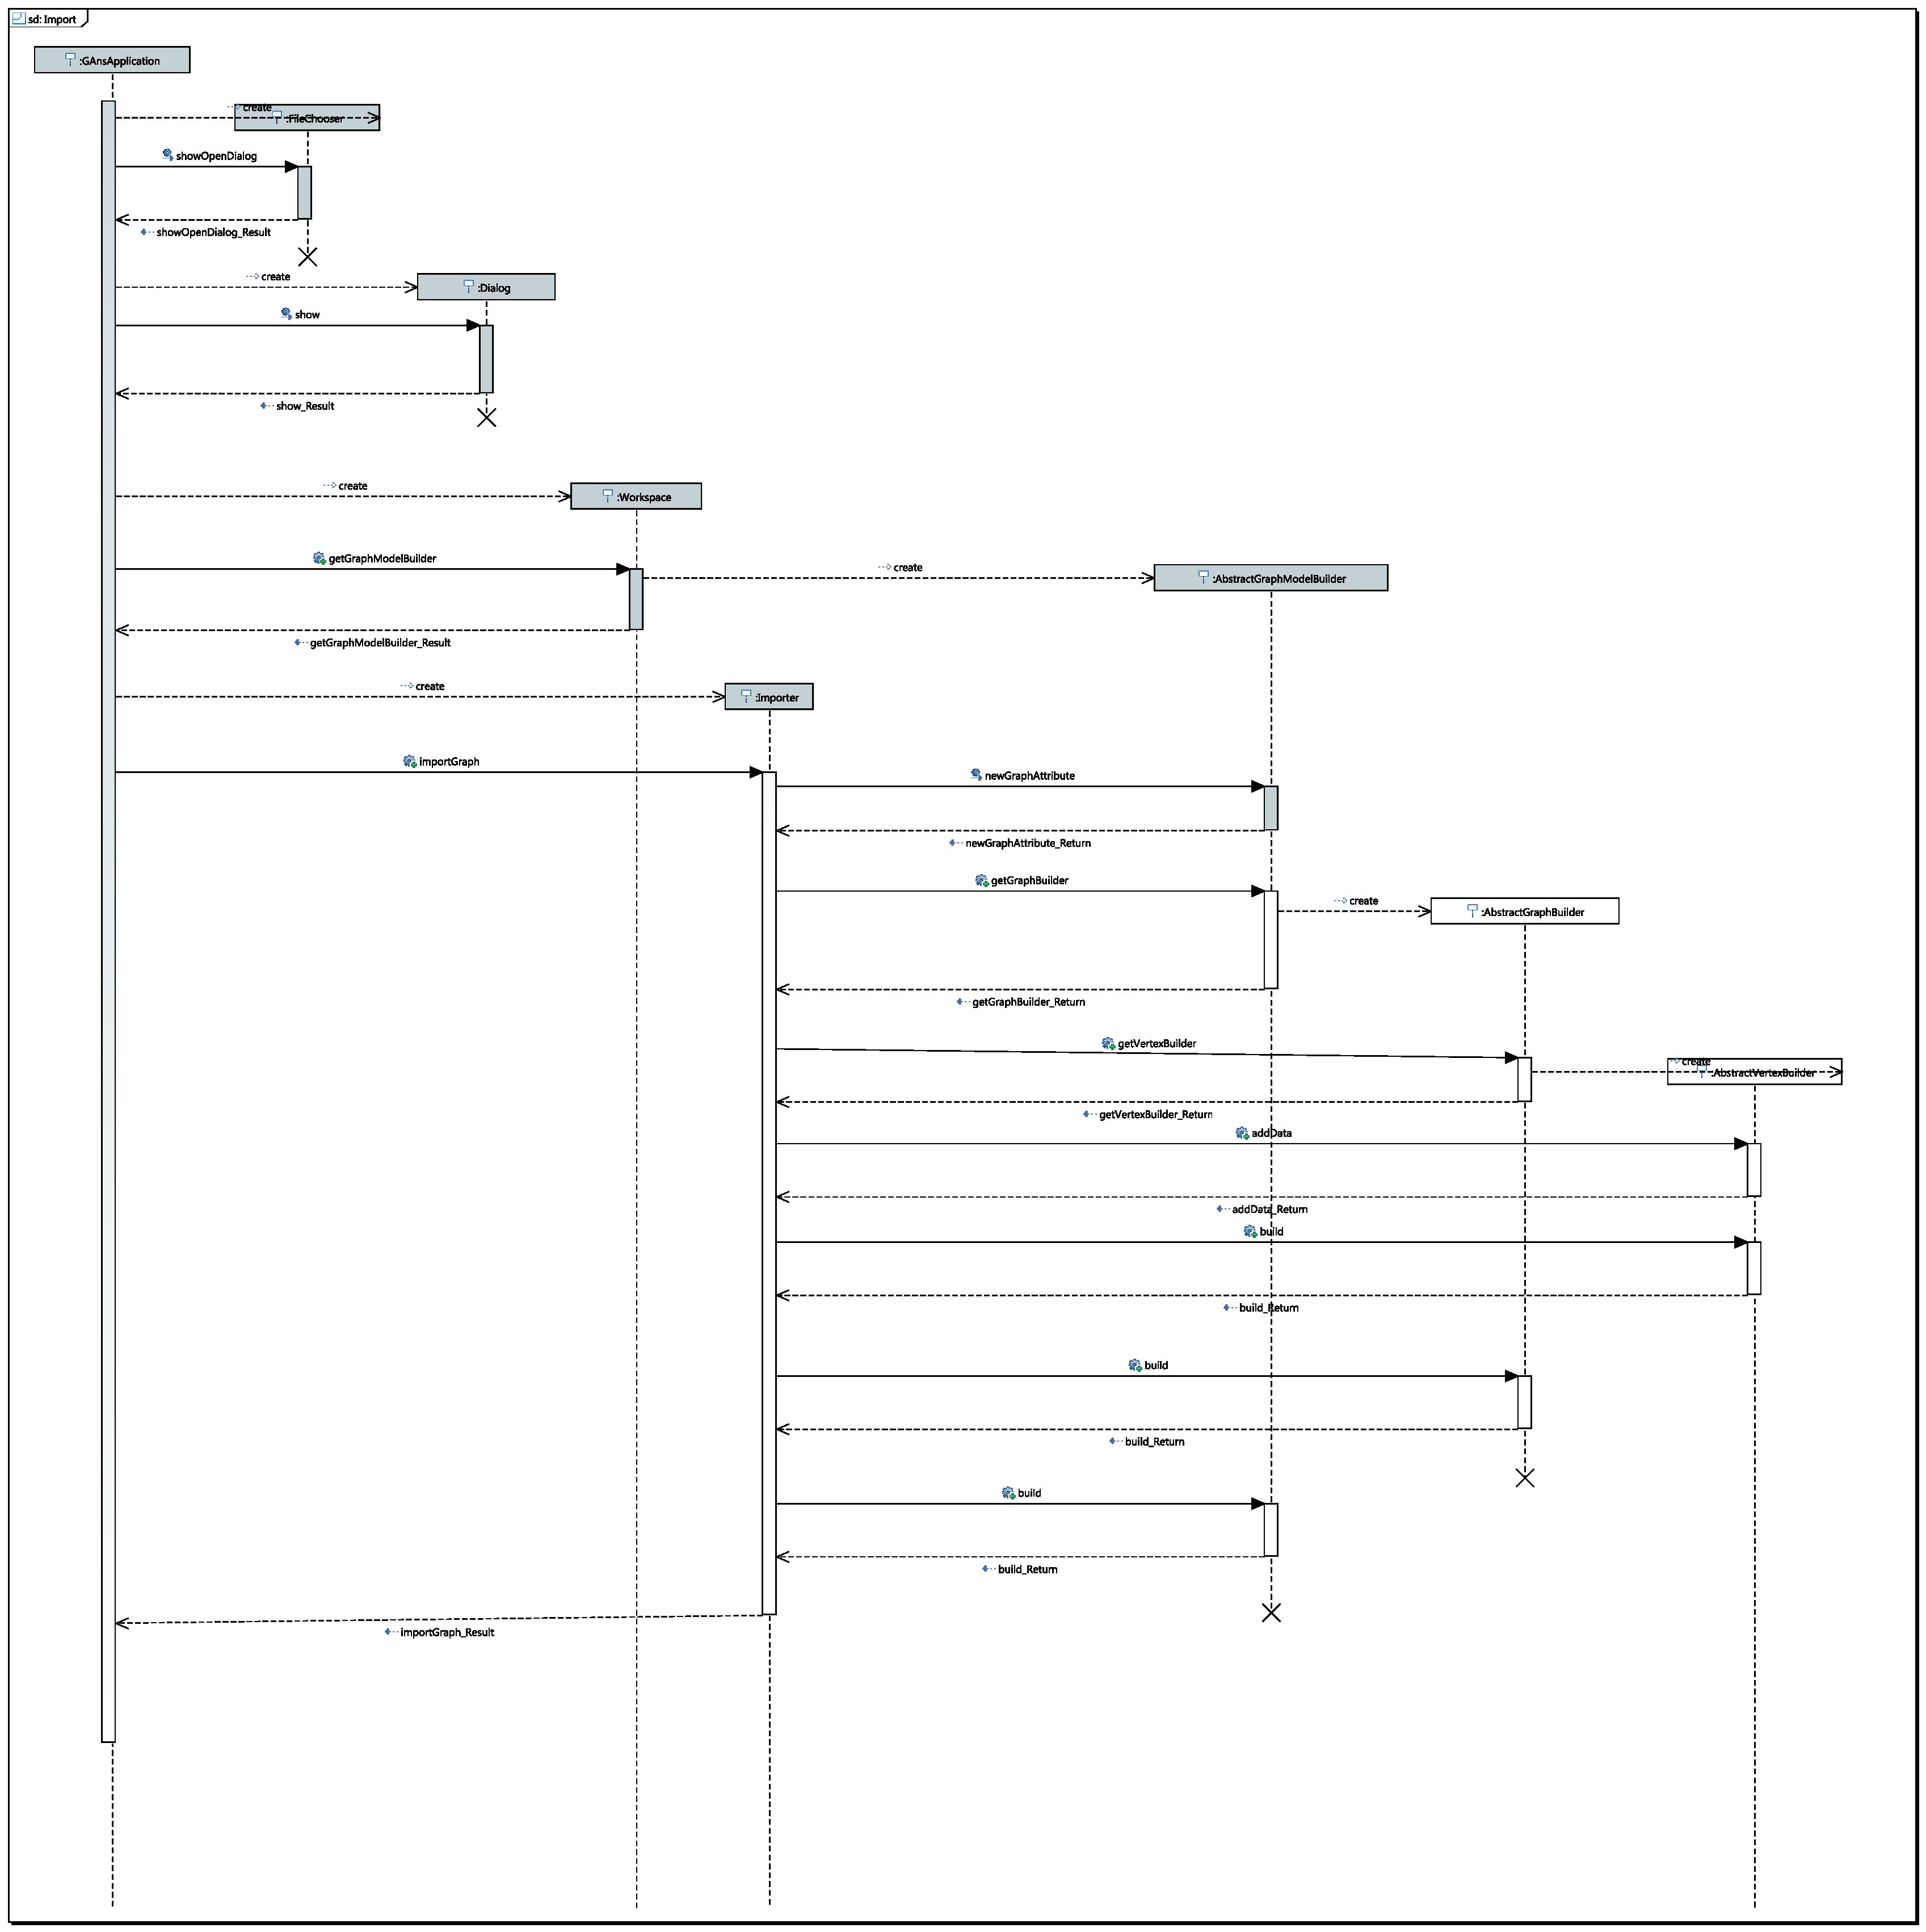
\includegraphics[width=450pt]{resourcen/SeqDiagramImport.PDF}
  \caption{Sequenz Diagramm für den Import}
  \label{seq:import}
\end{figure}

Der Benutzer möchte einen Graphen importieren und klickt auf Import. Die GAnsApplication öffnet einen FileChooser, in welchem der Benutzer die Datei auswählen kann welche er importieren möchte. Danach öffnet sich ein Workspace Dialog in welchem der Benutzer auswählt als welcher Typ der Graph interpretiert werden soll.\\
Das Workspace übergibt der GAnsApplication nun den dazugehörigen IGraphModelBuilder. Dieser wird dann dem Importer übergeben, welcher mithilfe des Builders eine Repräsentation des Graphen erstellt, welche Workspace spezifisch ist.

\section{Öffnen eines JOANA-Methodengraphen}
\begin{figure}[hb]
	\centering
	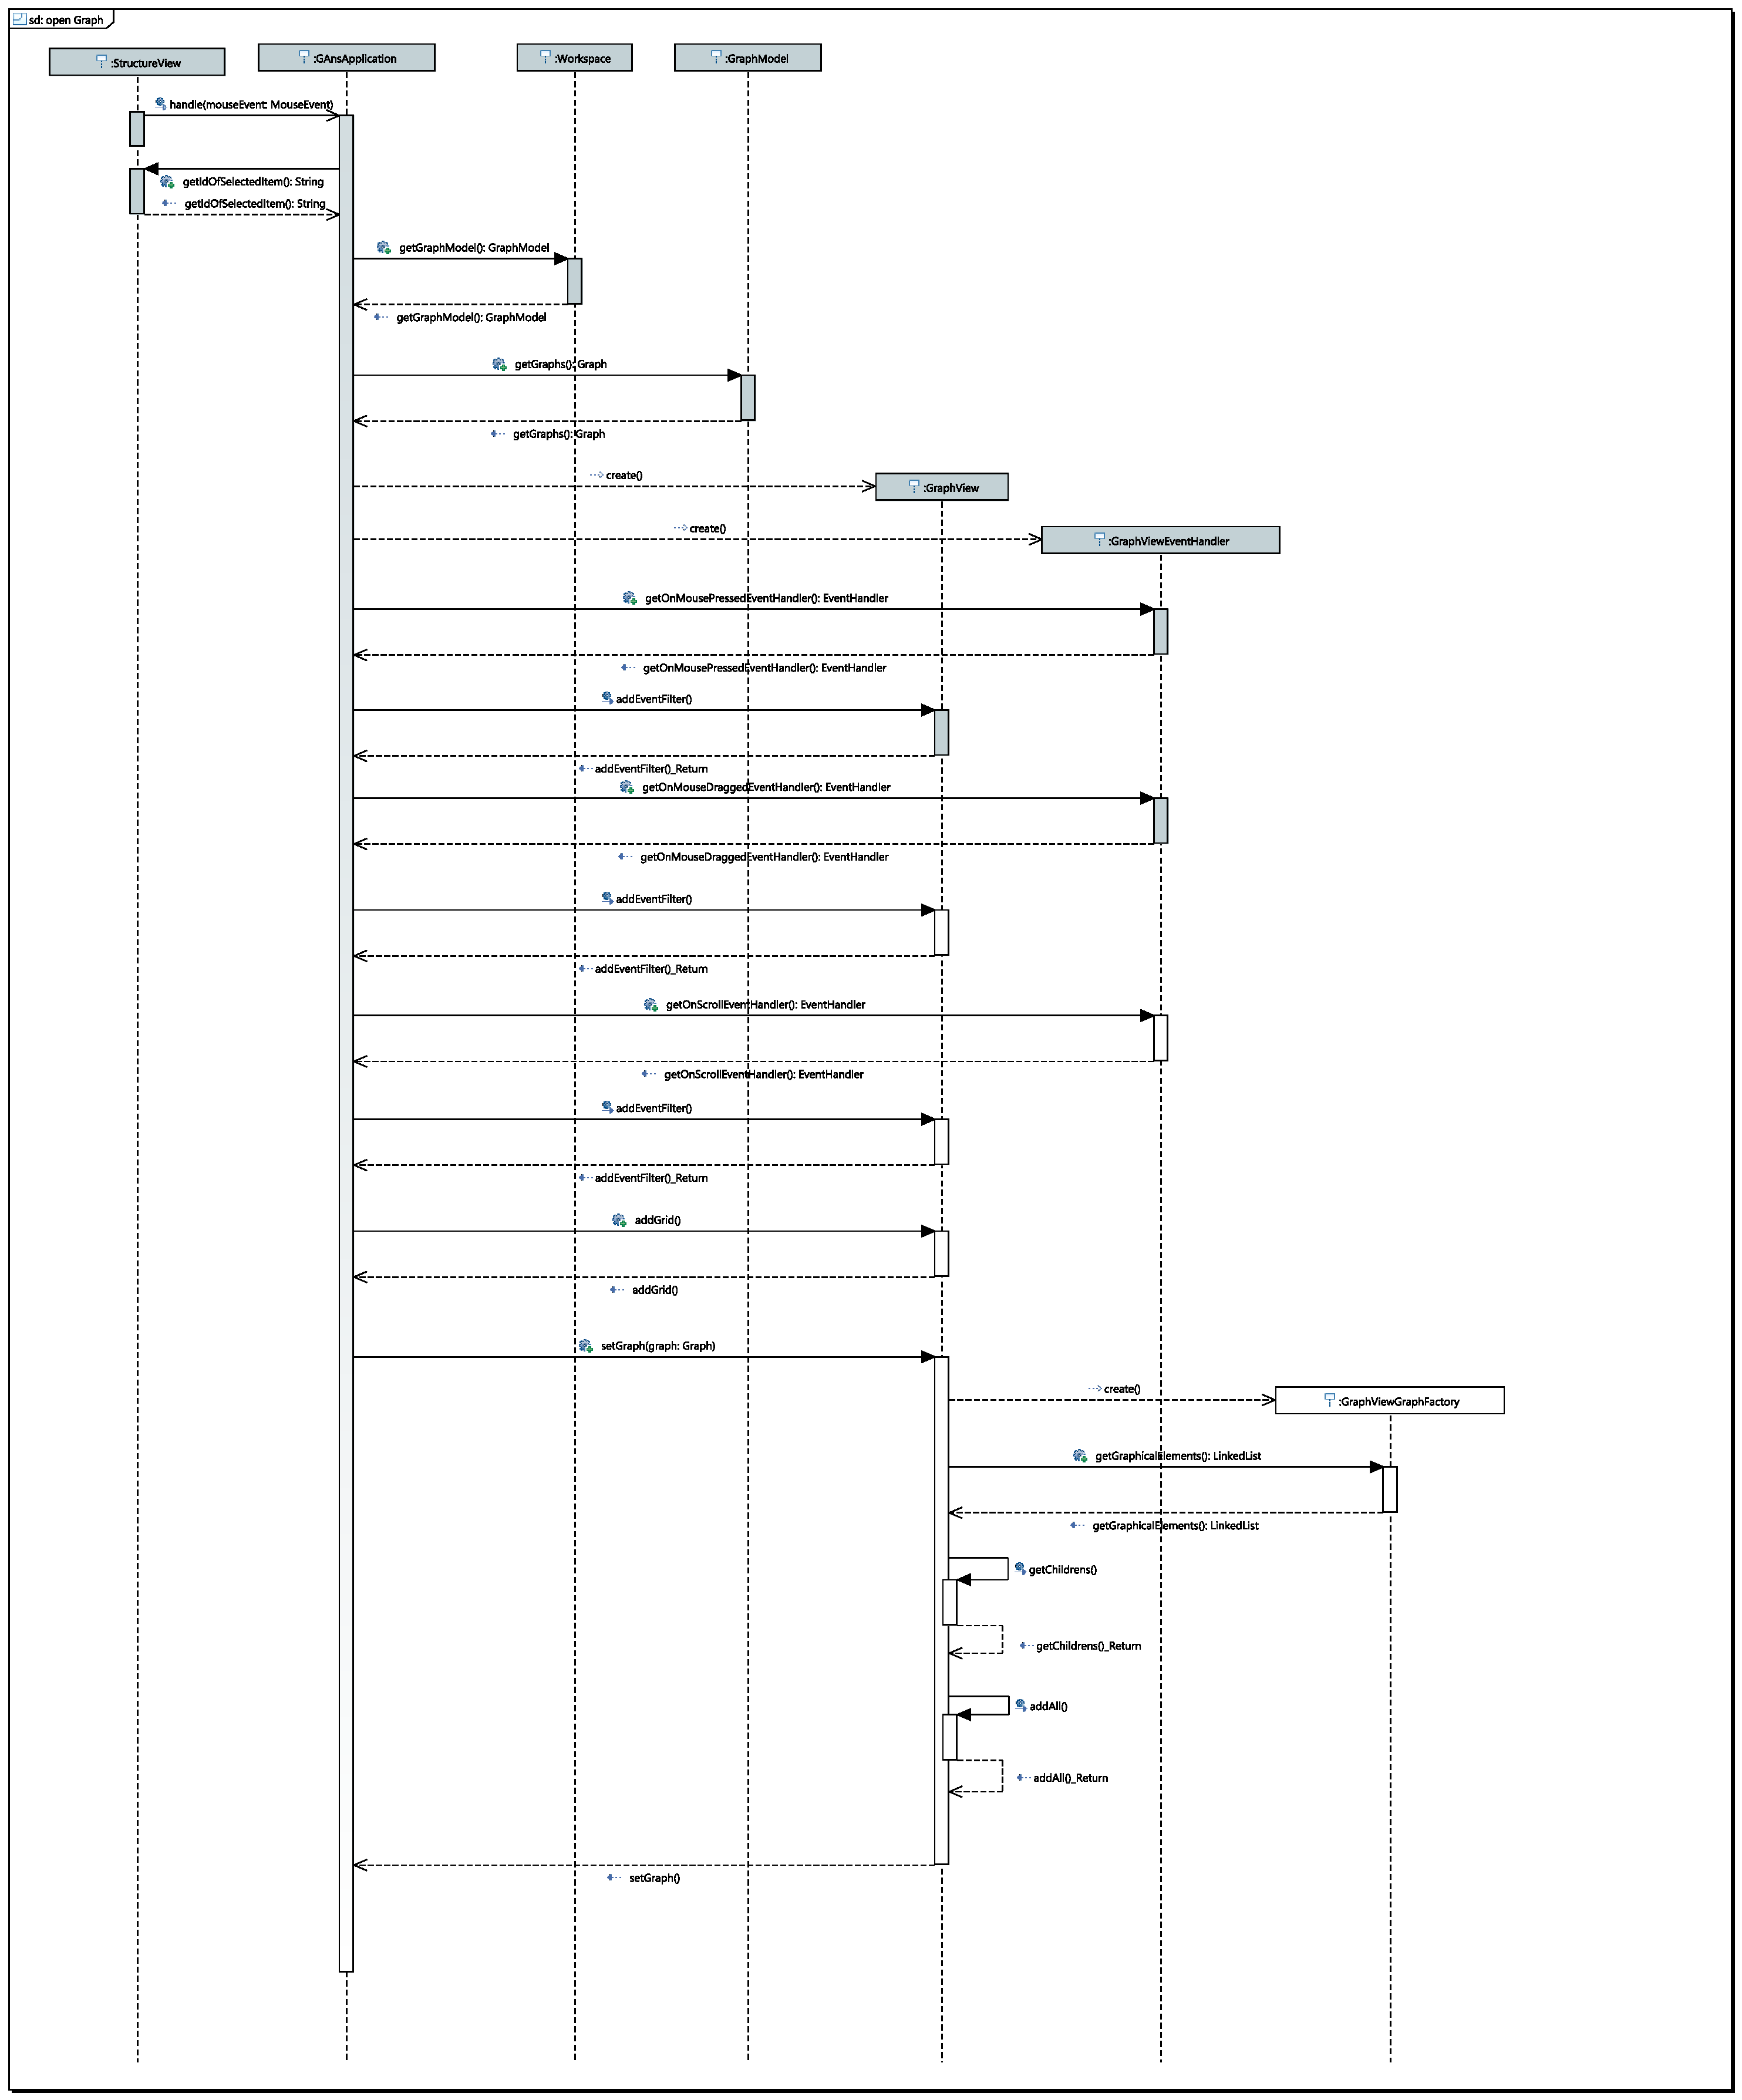
\includegraphics[width=450pt]{resourcen/SeqDiagramOpenGraph.PDF}
	\caption{Sequenz Diagramm das Öffnen eines Graphen aus der Strukturansicht}
	\label{seq:openMethod}
\end{figure}


\section{Ändern der Selektion im Graphen}
\begin{figure}[hb]
	\centering
	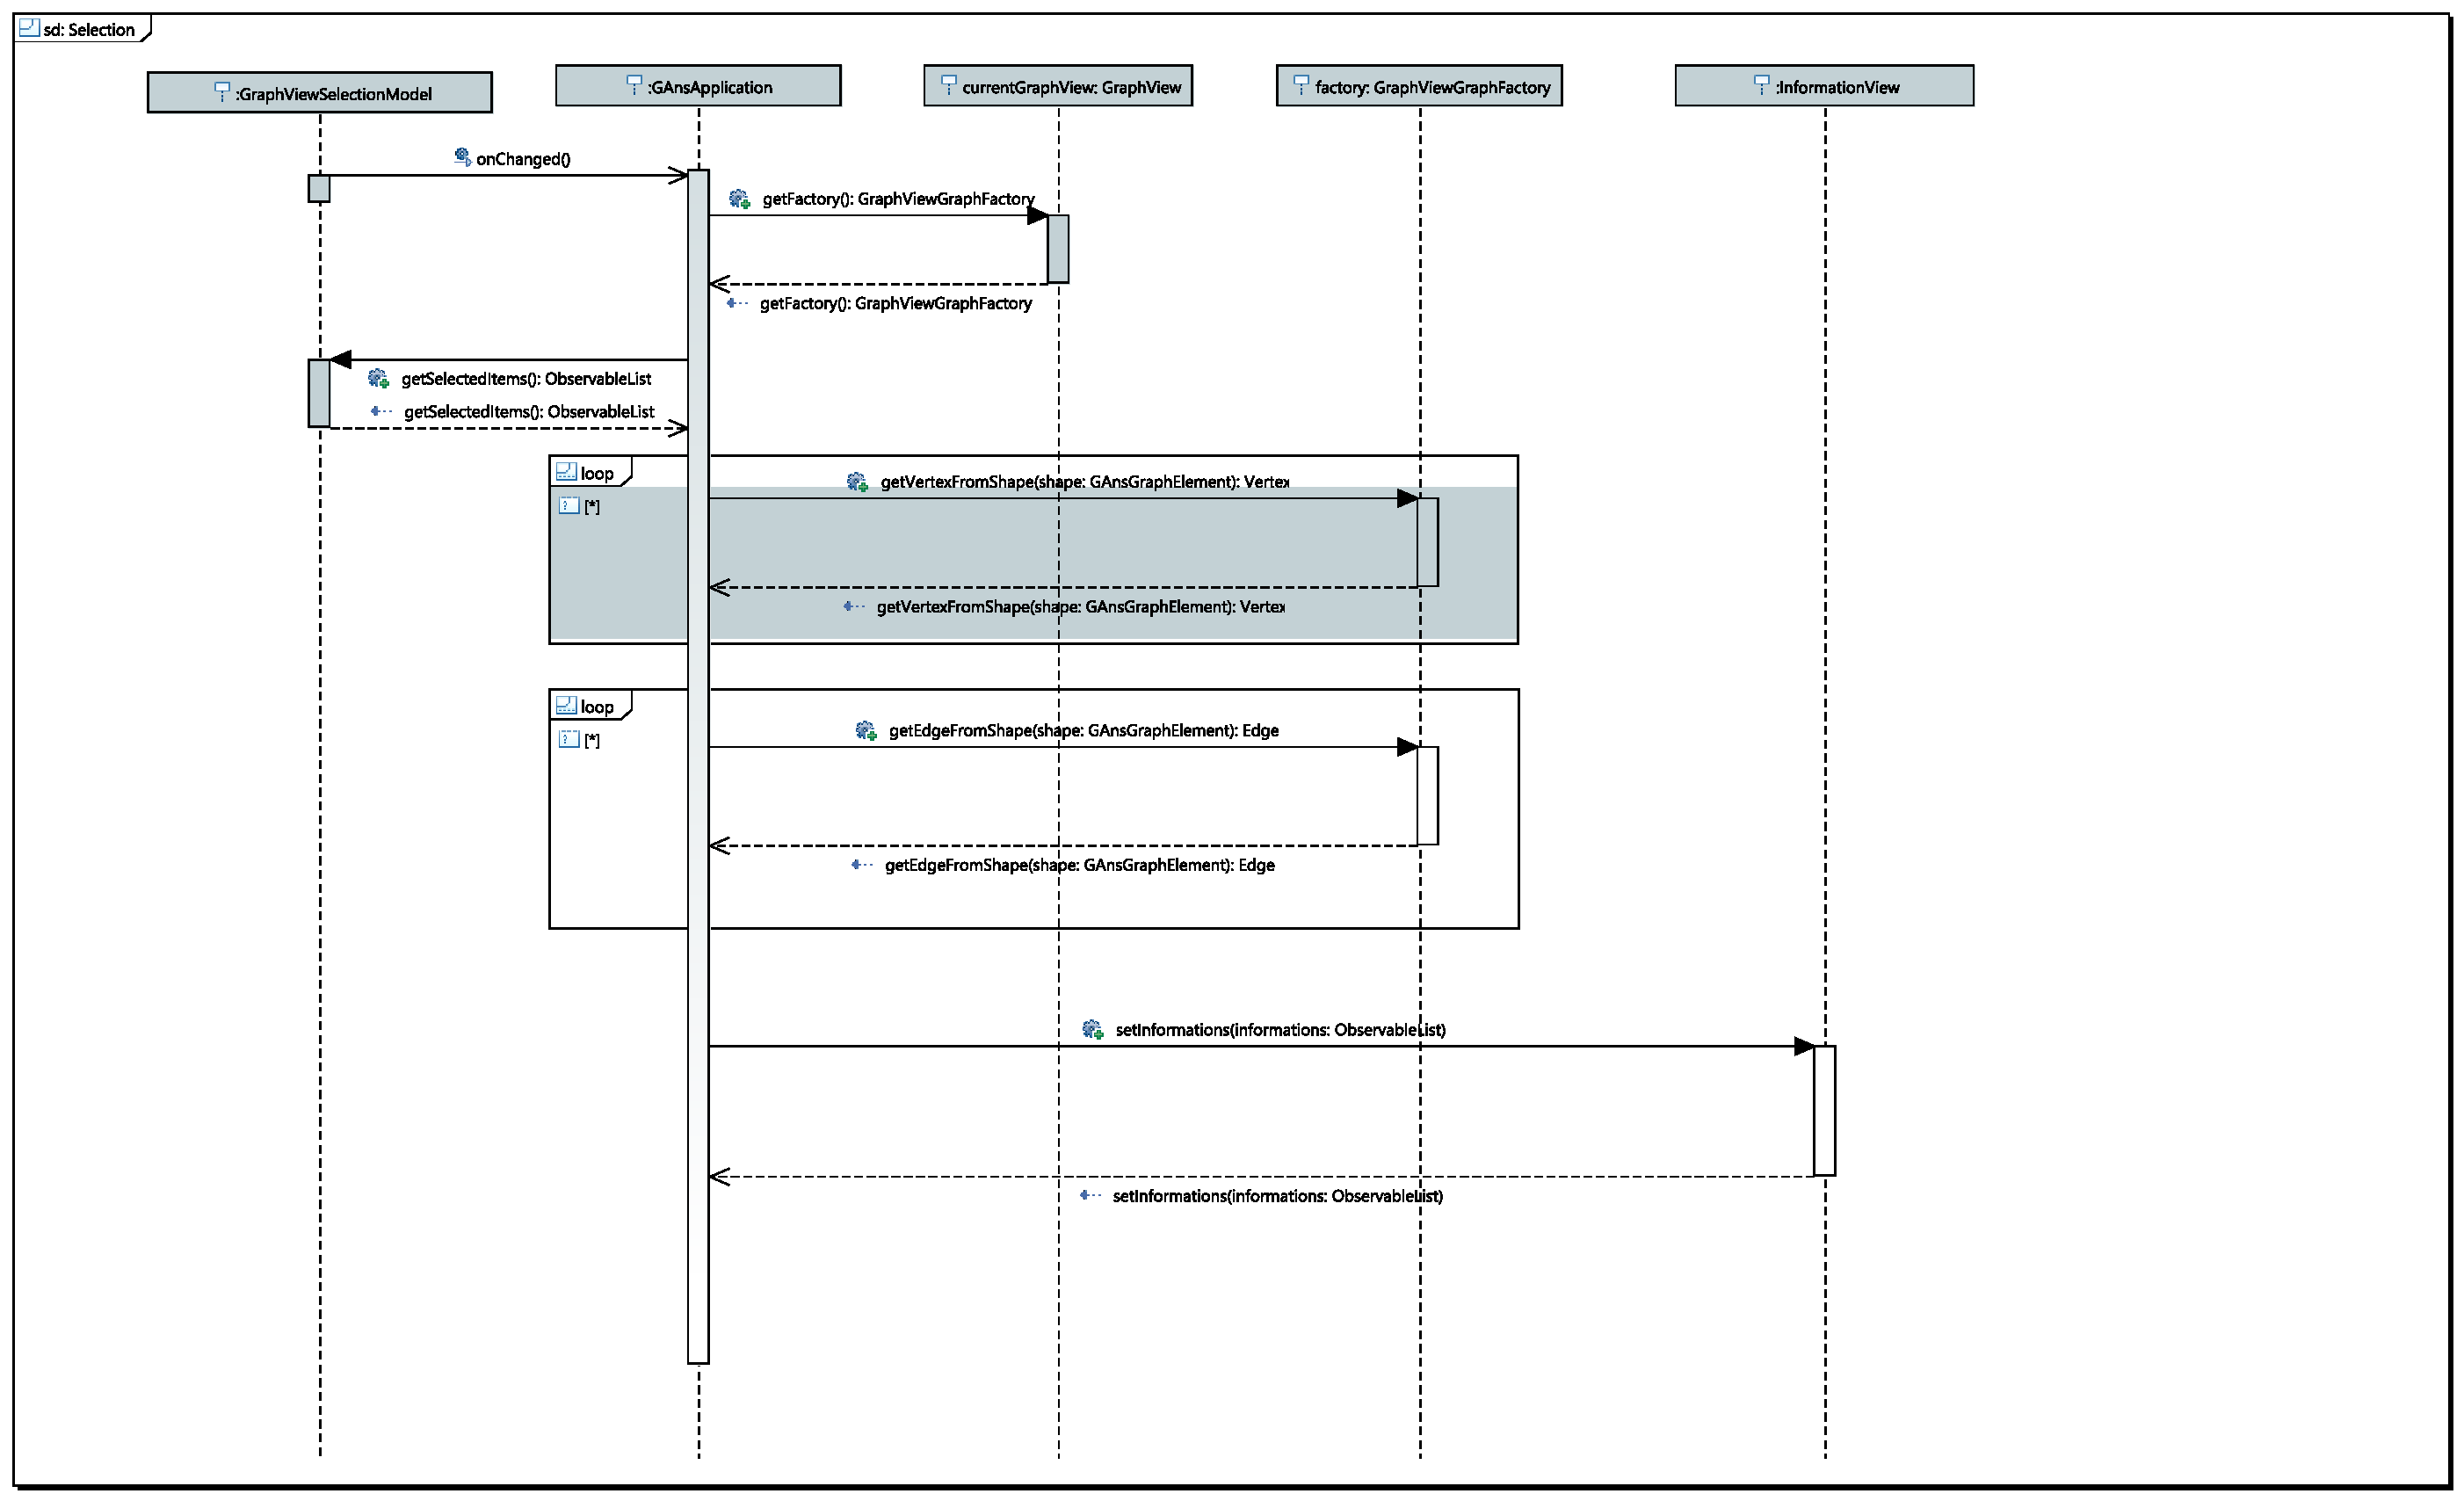
\includegraphics[width=450pt]{resourcen/SeqDiagramSelection.PDF}
	\caption{Sequenz Diagramm für geänderte Selektion}
	\label{seq:selection}
\end{figure}

Der Benutzer hat in der aktuellen GraphAnsicht die Selektion geändert. Die GAnsApplication wird vom GraphViewSelectionModel benachrichtigt. Die GAnsApplication holt sich von der aktuellen GraphAnsicht die Factory, welche zugriff auf die Elemente in der GraphView bietet, und vom SelectionModel eine Liste mit allen selektierten Elementen. Über die Factory und wird nun zu jedem selektiertem Element die zugehörige Vertex oder Edge aus dem angezeigten Graphen ermittelt. Deren GAnsProperties werden in eine ObservableList zusammengeführt und an die InformationsView übergeben, welche die Informationen die über die Properties gegeben sind darstellt.

\section{Navigation (Pflichtenheft 9 /T040/)}

\section{Filtern von Kanten (Pflichtenheft 9 /T060/)}

\section{Export von einem geladenen JOANA-Graphen als SVG (Pflichtenheft 9 /T070/)}